\documentclass[12pt,a4paper]{article}

% ============================================
% PACKAGES
% ============================================
\usepackage[utf8]{inputenc}
\usepackage[T1]{fontenc}
\usepackage{amsmath,amssymb}
\usepackage{booktabs}
\usepackage{longtable}
\usepackage{array}
\usepackage{multirow}
\usepackage{graphicx}
\usepackage{float}
\usepackage{caption}
\usepackage{geometry}
\usepackage{setspace}
\usepackage{parskip}
\usepackage{enumitem}
\usepackage{listings}
\usepackage{xcolor}
\usepackage{hyperref}
\usepackage{fancyhdr}
\usepackage{titlesec}
\usepackage{tocloft}
\usepackage{tikz}
\usetikzlibrary{arrows.meta, positioning, calc}

% ============================================
% TABLE OF CONTENTS FORMATTING
% ============================================
\setlength{\cftsecnumwidth}{3em}
\setlength{\cftsubsecnumwidth}{3.5em}
\setlength{\cftsubsubsecnumwidth}{4.5em}

% ============================================
% PAGE LAYOUT
% ============================================
\geometry{
    left=1.5in,
    right=1in,
    top=1in,
    bottom=1in
}

% ============================================
% LINE SPACING
% ============================================
\onehalfspacing

% ============================================
% HEADER AND FOOTER — page numbers at bottom centre
% ============================================
\pagestyle{fancy}
\fancyhf{}
\fancyfoot[C]{\thepage}
\renewcommand{\headrulewidth}{0pt}
\renewcommand{\footrulewidth}{0pt}

% ============================================
% SECTION FORMATTING
% ============================================
\titleformat{\section}
    {\normalfont\Large\bfseries}{\thesection}{1em}{}
\titleformat{\subsection}
    {\normalfont\large\bfseries}{\thesubsection}{1em}{}
\titleformat{\subsubsection}
    {\normalfont\normalsize\bfseries}{\thesubsubsection}{1em}{}

% ============================================
% CODE LISTING STYLE
% ============================================
\definecolor{codegreen}{rgb}{0,0.6,0}
\definecolor{codegray}{rgb}{0.5,0.5,0.5}
\definecolor{codepurple}{rgb}{0.58,0,0.82}
\definecolor{backcolour}{rgb}{0.95,0.95,0.92}

\lstdefinestyle{mystyle}{
    backgroundcolor=\color{backcolour},
    commentstyle=\color{codegreen},
    keywordstyle=\color{blue},
    numberstyle=\tiny\color{codegray},
    stringstyle=\color{codepurple},
    basicstyle=\ttfamily\footnotesize,
    breakatwhitespace=false,
    breaklines=true,
    captionpos=b,
    keepspaces=true,
    numbers=left,
    numbersep=5pt,
    showspaces=false,
    showstringspaces=false,
    showtabs=false,
    tabsize=2,
    frame=single
}
\lstset{style=mystyle}

% ============================================
% HYPERREF SETUP
% ============================================
\hypersetup{
    colorlinks=true,
    linkcolor=blue,
    filecolor=magenta,
    urlcolor=cyan,
    citecolor=blue,
    pdftitle={Mitiga Global Analytics Engine: Physical Climate Risk Prototype},
    pdfauthor={Kuwana Tadiwanaishe J},
    bookmarks=true,
}

% ============================================
% CUSTOM COMMANDS
% ============================================
\newcommand{\Mnormal}{M_{\text{normal}}}
\newcommand{\Mstress}{M_{\text{stress}}}
\newcommand{\ECL}{\text{ECL}}
\newcommand{\EAD}{\text{EAD}}
\newcommand{\LGD}{\text{LGD}}
\newcommand{\PD}{\text{PD}}

% ============================================
% WIREFRAME COLOURS
% ============================================
\definecolor{wfgreen}{RGB}{4,120,87}
\definecolor{wfgreenlt}{RGB}{209,250,229}
\definecolor{wfgray}{RGB}{248,250,252}
\definecolor{wfborder}{RGB}{203,213,225}
\definecolor{wfblue}{RGB}{239,246,255}
\definecolor{wfred}{RGB}{254,242,242}
\definecolor{wfamber}{RGB}{255,251,235}
\definecolor{wfdark}{RGB}{15,23,42}
\definecolor{wfnavbg}{RGB}{255,255,255}
\definecolor{wfstatbg}{RGB}{15,23,42}
\definecolor{wfbadgered}{RGB}{239,68,68}
\definecolor{wfbadgegreen}{RGB}{16,185,129}
\definecolor{wfbadgeamber}{RGB}{245,158,11}

% ============================================
% DOCUMENT BEGIN
% ============================================
\begin{document}

% ============================================
% COVER PAGE (not numbered)
% ============================================
\thispagestyle{empty}
\begin{center}


\includegraphics[width=0.5\textwidth]{hit_logo.png}

\vspace{0.3cm}

{\normalsize\bfseries SCHOOL OF BUSINESS AND MANAGEMENT SCIENCES}\\[0.2cm]
{\normalsize\bfseries DEPARTMENT OF FINANCIAL ENGINEERING}

\vspace{1.5cm}

{\large\bfseries MITIGA GLOBAL ANALYTICS ENGINE}

\vspace{1.5cm}

{\normalsize BY}

\vspace{0.5cm}

{\large\bfseries KUWANA TADIWANAISHE J}\\[0.2cm]
{\large\bfseries H220006Z}

\vspace{1cm}

{\normalsize SUPERVISOR: MR MANGWANDA}

\vspace{1cm}

{\small THIS PROTOTYPE IS SUBMITTED TO THE DEPARTMENT OF FINANCIAL ENGINEERING, SCHOOL OF BUSINESS AND MANAGEMENT SCIENCES, IN PARTIAL FULLFILLMENT OF THE BACHELOR OF TECHNOLOGY HONOURS DEGREE IN FINANCIAL ENGINEERING}

\vspace{1cm}

{\large\bfseries 2026}

\end{center}

\newpage

% ============================================
% FRONT MATTER — Roman numerals, bottom centre
% ============================================
\pagenumbering{roman}
\setcounter{page}{1}

% ============================================
% TITLE PAGE  (i)
% ============================================
\phantomsection
\addcontentsline{toc}{section}{Title Page}
\thispagestyle{fancy}

\section*{Title Page}

\vspace{0.5cm}

\begin{tabular}{p{4.2cm} p{8cm}}
\textbf{Title of project:}   & MITIGA GLOBAL ANALYTICS ENGINE \\[0.9cm]
\textbf{Author:}              & KUWANA TADIWANAISHE J \\[0.9cm]
\textbf{University Name:}     & HARARE INSTITUTE OF TECHNOLOGY \\[0.9cm]
\textbf{School Name:}         & BUSINESS AND MANAGEMENT SCIENCES \\[0.9cm]
\textbf{Department Name:}     & DEPARTMENT OF FINANCIAL ENGINEERING \\[0.9cm]
\textbf{Year:}                & 2026 \\
\end{tabular}

\newpage

% ============================================
% DECLARATION  (ii)
% ============================================
\phantomsection
\addcontentsline{toc}{section}{Declaration}
\section*{Declaration}

I the author, KUWANA TADIWANAISHE J H220006Z do hereby declare that this work has not previously been accepted in substance for any degree and is not being concurrently submitted in candidature for any degree.

\vspace{2.5cm}

Student Signature\dotfill Date\dotfill

\vspace{2.5cm}

Supervisor's Signature\dotfill Date\dotfill

\newpage

% ============================================
% COPYRIGHT  (iii)
% ============================================
\phantomsection
\addcontentsline{toc}{section}{Copyright}
\section*{Copyright}

All rights reserved. No part of this research may be reproduced, stored in any retrieval system, or transmitted in any form or by any means, electronic, mechanical, photocopying, recording or otherwise from scholarly purpose without the prior written permission of the author and Harare Institute of Technology on behalf of the author.

\newpage

% ============================================
% DEDICATION  (iv)
% ============================================
\phantomsection
\addcontentsline{toc}{section}{Dedication}
\section*{Dedication}

This prototype is dedicated to my mother and father, who supported my education every step of the way. My brothers and friends kept me going when things got hard. This one is for all of you.

\newpage

% ============================================
% ACKNOWLEDGEMENTS  (v)
% ============================================
\phantomsection
\addcontentsline{toc}{section}{Acknowledgements}
\section*{Acknowledgements}

I would like to thank Mr Mangwanda for his guidance and steady support throughout this project. His feedback was always clear and practical. It made a real difference.

I also thank the research coordinators in the Department of Financial Engineering. Their structure and direction kept the project on track, especially in the later stages when things got complicated.

To my friends at HIT --- four years went fast. The things we learned together, inside and outside the classroom, I will carry for a long time. Thank you.

\newpage

% ============================================
% TABLE OF CONTENTS
% ============================================
\tableofcontents
\newpage

% ============================================
% LIST OF FIGURES
% ============================================
\listoffigures
\newpage

% ============================================
% LIST OF TABLES
% ============================================
\listoftables
\newpage

% ============================================
% ABSTRACT  (x)
% ============================================
\phantomsection
\addcontentsline{toc}{section}{Abstract}
\section*{Abstract}

The Mitiga Global Analytics Engine is a web-based prototype that implements the research findings from the dissertation on physical climate risk in Zimbabwe's microfinance sector. The system brings the Two-Regime Markov-Switching credit migration model to life as a working application. Satellite data from Google Earth Engine is used to compute NDVI-based agricultural health scores and a field-level drought index ($\gamma$) for each registered borrower. This drought index drives the logistic regime weight $\omega(\gamma)$, which blends the normal and drought-stress migration matrices to produce a dynamic Probability of Default. From there, the system computes IFRS 9-compliant Expected Credit Loss across four forward-looking scenarios. Credit officers can manage the full borrower lifecycle through an admin dashboard, while farmers access a simplified view of their farm health and loan status. The prototype demonstrates that the theoretical framework is not only mathematically valid but also operationally feasible.

\newpage

% ============================================
% ABBREVIATION  (xi)
% ============================================
\phantomsection
\addcontentsline{toc}{section}{Abbreviation}
\section*{Abbreviation}

\begin{center}
\begin{tabular}{|p{3.5cm}|p{9cm}|}
\hline
\textbf{Abbreviation} & \textbf{Full Form} \\
\hline
IFRS 9   & International Financial Reporting Standard 9 \\
\hline
ECL      & Expected Credit Loss \\
\hline
PD       & Probability of Default \\
\hline
LGD      & Loss Given Default \\
\hline
EAD      & Exposure at Default \\
\hline
SPEI     & Standardized Precipitation Evapotranspiration Index \\
\hline
NDVI     & Normalized Difference Vegetation Index \\
\hline
GEE      & Google Earth Engine \\
\hline
MFI      & Microfinance Institution \\
\hline
API      & Application Programming Interface \\
\hline
UI       & User Interface \\
\hline
TTC      & Through-the-Cycle \\
\hline
PIT      & Point-in-Time \\
\hline
\end{tabular}
\captionof{table}{Glossary of Abbreviations}
\end{center}

\newpage

% ============================================
% BODY — Arabic numerals, bottom centre
% ============================================
\hypersetup{pageanchor=false}
\pagenumbering{arabic}
\setcounter{page}{1}
\hypersetup{pageanchor=true}

% ============================================
% CHAPTER 1: INTRODUCTION
% ============================================
\begin{center}
    {\large\bfseries Chapter 1}\\[0.5cm]
    {\LARGE\bfseries INTRODUCTION}
\end{center}
\phantomsection
\addcontentsline{toc}{section}{Chapter 1: Introduction}

\vspace{0.8cm}

The research dissertation validated the Two-Regime Markov-Switching model as a rigorous approach to estimating Expected Credit Loss under physical climate risk. Chapter 4 of the study showed that conditioning credit migration on the drought index produces materially different default probabilities during stress periods, with the AUC improving from 0.618 under the static single-matrix model to 0.724 under the two-regime model. The Mitiga Global Analytics Engine takes that validated framework and turns it into a working web application. Credit officers can register borrowers, map their farmland, retrieve satellite NDVI data from Google Earth Engine, and compute a field-level drought gamma for each farm. The system then applies the regime-switching logic to estimate ECL under four IFRS 9-compliant forward-looking scenarios.

\setcounter{section}{0}
\renewcommand{\thesection}{1.\arabic{section}}

\section{Problem Statement}

Microfinance Institutions in Zimbabwe face a very specific credit risk problem. Most of their borrowers are smallholder farmers. When drought hits, repayment capacity drops sharply and it does not happen gradually --- it happens all at once, across the whole portfolio. Static credit risk models miss this completely. They estimate an average probability of default that stays the same regardless of whether the region is wet or dry. The result is chronic under-provisioning during exactly the periods when losses are highest.

The research quantified this gap. Portfolio ECL under the two-regime model was significantly higher during drought conditions than the figure produced by the static model. That difference represents real capital exposure that MFIs are currently ignoring. Without a tool that implements the regime-switching logic, credit officers have no way to convert a satellite drought reading into an IFRS 9 loss estimate. The Mitiga Global Analytics Engine was built to close that gap.

\section{System Objectives}

The prototype was built to meet the following specific objectives:

\begin{itemize}[noitemsep]
    \item To allow credit officers to register and manage microfinance borrowers, linking each to their registered farm field
    \item To use Google Earth Engine to fetch NDVI and weather data for drawn farm polygons, and to compute a field-level agricultural health score (0--100)
    \item To derive a drought index $\gamma$ from the health score and apply the logistic regime weight $\omega(\gamma)$ to blend $\Mnormal$ and $\Mstress$ migration matrices
    \item To compute 1-year and lifetime ECL under four IFRS 9 scenarios: baseline, moderate drought, severe drought, and wet recovery
    \item To aggregate individual borrower risk into a portfolio view showing regime distribution and scenario-weighted ECL
    \item To provide borrowers with a plain-language dashboard showing their farm health score and loan risk status
\end{itemize}

\subsection*{Conclusion}

The Mitiga Global Analytics Engine makes the research framework operational. Every step in the system --- from the GEE satellite fetch to the final ECL figure --- maps directly to equations and parameters from the dissertation. The chapters that follow explain how the system was designed, what process model was used, and how each screen in the application works.

\newpage

% ============================================
% CHAPTER 2: PROCESS MODELLING
% ============================================
\begin{center}
    {\large\bfseries Chapter 2}\\[0.5cm]
    {\LARGE\bfseries PROCESS MODELLING}
\end{center}
\phantomsection
\addcontentsline{toc}{section}{Chapter 2: Process Modelling}

\vspace{0.8cm}

\setcounter{section}{0}
\renewcommand{\thesection}{2.\arabic{section}}

\section{Introduction}

The system was built using an iterative prototyping approach. This was a deliberate decision. The Two-Regime Markov-Switching model at the core of the application has several interacting parameters --- the regime sharpness $\kappa$, the drought threshold $\gamma_0$, the LGD assumption, and the structure of the two migration matrices. Getting those parameters to produce sensible outputs required building early versions and testing them against known results from the dissertation. A waterfall approach would have locked the design in too early. Iteration was the only practical path.

\section{Process Model (Iterative)}

\begin{figure}[H]
\centering
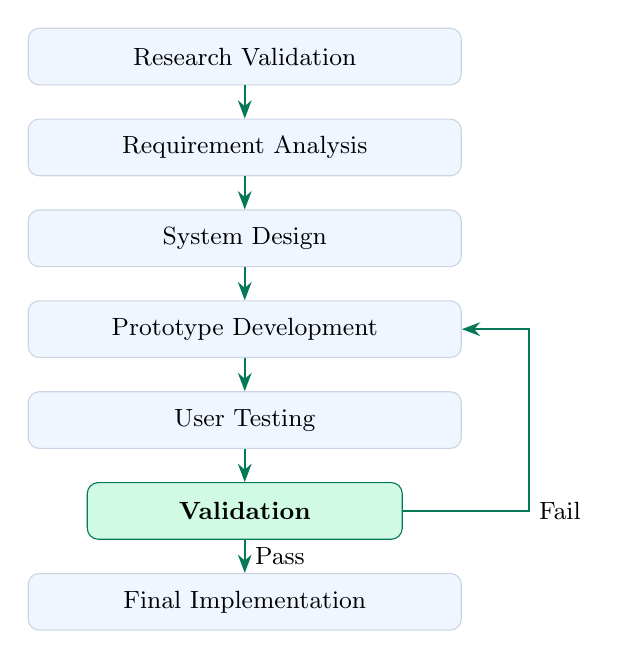
\begin{tikzpicture}[
    box/.style={rectangle, draw=wfborder, rounded corners=4pt, fill=wfblue,
        minimum width=5.5cm, minimum height=0.72cm, text centered, font=\small},
    valbox/.style={rectangle, draw=wfgreen, rounded corners=4pt,
        fill=wfgreenlt, minimum width=4cm, minimum height=0.72cm,
        text centered, font=\small\bfseries},
    arrow/.style={-Stealth, thick, color=wfgreen}
]
\node[box]    (research) {Research Validation};
\node[box, below=0.42cm of research] (req)    {Requirement Analysis};
\node[box, below=0.42cm of req]      (design) {System Design};
\node[box, below=0.42cm of design]   (dev)    {Prototype Development};
\node[box, below=0.42cm of dev]      (test)   {User Testing};
\node[valbox, below=0.42cm of test]  (val)    {Validation};
\node[box, below=0.42cm of val]      (final)  {Final Implementation};

\draw[arrow] (research) -- (req);
\draw[arrow] (req)      -- (design);
\draw[arrow] (design)   -- (dev);
\draw[arrow] (dev)      -- (test);
\draw[arrow] (test)     -- (val);
\draw[arrow] (val)      -- node[right, font=\small, color=black]{Pass} (final);
\draw[arrow] (val.east) -- ++(1.6,0) node[right, font=\small, color=black]{Fail}
             |- (dev.east);
\end{tikzpicture}
\caption{Process Model (Iterative)}
\label{fig:process_model}
\end{figure}

The iterative model was the right fit for three reasons. First, the regime parameters needed real calibration cycles. The threshold value $\gamma_0 = -1.10$ was arrived at after testing several values against the dissertation's empirical data. Getting it wrong early would have produced wrong ECL numbers throughout. Second, the Next.js web stack supported fast iteration --- a change to the API or a UI fix was live in seconds, which kept development moving. Third, the borrower registration and field analysis workflow went through several revisions based on test runs. Each time it became simpler. That kind of refinement only happens when you build, test, and build again.

\section{Feasibility Analysis}

\begin{itemize}[noitemsep]
    \item \textbf{Economic Feasibility}: The entire system uses open-source technologies. Next.js, Prisma, SQLite, and TypeScript are all free. Google Earth Engine provides satellite data at no cost for academic use. There are no licensing fees anywhere in the stack.

    \item \textbf{Technical Feasibility}: The regime-switching computation is not expensive. The logistic weight $\omega(\gamma)$, the matrix blending, and the ECL summation all run in milliseconds inside Next.js API routes. There is no need for a dedicated compute server. A standard laptop or small cloud instance is sufficient.

    \item \textbf{Social Feasibility}: The system serves two very different users. Credit officers are comfortable with tables and numbers --- the admin dashboard reflects that. Borrowers are farmers who may not be comfortable with financial terminology --- the borrower dashboard is intentionally stripped of technical language. Both groups were considered separately from the start.

    \item \textbf{Operational Feasibility}: The system is a web application. Any device with a browser can use it. No installation is required on the user side. The SQLite database keeps the backend simple with no external database server to configure.
\end{itemize}

\section{System Security}

The system has two layers of security. The first is role-based access control. There is no public signup for credit officers --- admin accounts are created directly by the system developer. Borrowers can register through a public page but can only see their own data once logged in. The second layer is password security. All passwords are stored as bcrypt hashes. Sessions use HTTP-only cookies which cannot be read by client-side JavaScript. Every protected page checks the session and user role on the server side before rendering anything.

\subsection*{Conclusion}

Iterative prototyping gave the flexibility needed to calibrate model parameters and refine the user interface through repeated cycles of building and testing. The feasibility study shows the system is economically and technically practical. Security is handled at the authentication layer with role separation and secure session management. The next chapter covers the actual application screens and how they implement the research framework.

\newpage

% ============================================
% CHAPTER 3: SOFTWARE METHODOLOGY
% ============================================
\begin{center}
    {\large\bfseries Chapter 3}\\[0.5cm]
    {\LARGE\bfseries SOFTWARE METHODOLOGY}
\end{center}
\phantomsection
\addcontentsline{toc}{section}{Chapter 3: Software Methodology}

\vspace{0.8cm}

\setcounter{section}{0}
\renewcommand{\thesection}{3.\arabic{section}}

\section{Introduction}

This chapter describes the system from the user's side. Each main screen is presented and explained. The Mitiga Global Analytics Engine is a Next.js web application backed by a Prisma ORM and a SQLite database. It has two user roles: Administrator (the credit officer) and Borrower (the farmer). Each role sees a different part of the system. Wireframes and screen descriptions are given below.

\section{System Flowchart}

\begin{figure}[H]
\centering
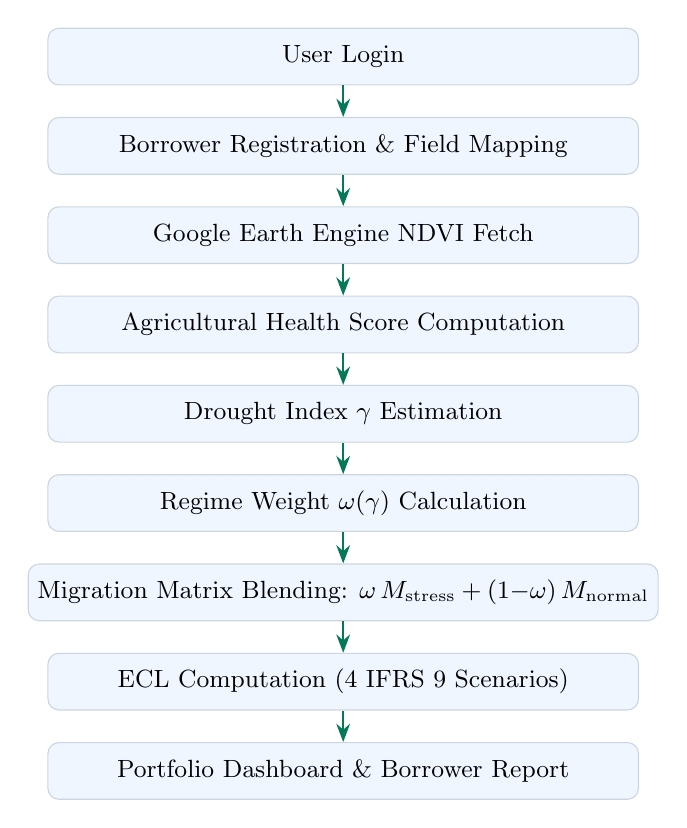
\begin{tikzpicture}[
    box/.style={rectangle, draw=wfborder, rounded corners=4pt, fill=wfblue,
        minimum width=7.5cm, minimum height=0.72cm, text centered, font=\small},
    arrow/.style={-Stealth, thick, color=wfgreen}
]
\node[box] (login)  {User Login};
\node[box, below=0.40cm of login]  (reg)    {Borrower Registration \& Field Mapping};
\node[box, below=0.40cm of reg]    (gee)    {Google Earth Engine NDVI Fetch};
\node[box, below=0.40cm of gee]    (score)  {Agricultural Health Score Computation};
\node[box, below=0.40cm of score]  (gamma)  {Drought Index $\gamma$ Estimation};
\node[box, below=0.40cm of gamma]  (weight) {Regime Weight $\omega(\gamma)$ Calculation};
\node[box, below=0.40cm of weight] (matrix) {Migration Matrix Blending: $\omega\,\Mstress + (1{-}\omega)\,\Mnormal$};
\node[box, below=0.40cm of matrix] (ecl)    {ECL Computation (4 IFRS 9 Scenarios)};
\node[box, below=0.40cm of ecl]    (report) {Portfolio Dashboard \& Borrower Report};

\draw[arrow] (login)  -- (reg);
\draw[arrow] (reg)    -- (gee);
\draw[arrow] (gee)    -- (score);
\draw[arrow] (score)  -- (gamma);
\draw[arrow] (gamma)  -- (weight);
\draw[arrow] (weight) -- (matrix);
\draw[arrow] (matrix) -- (ecl);
\draw[arrow] (ecl)    -- (report);
\end{tikzpicture}
\caption{System Flowchart}
\label{fig:system_flowchart}
\end{figure}

The flowchart traces the data from login all the way to the portfolio report. The Google Earth Engine step is the critical one. It pulls NDVI and 14-day weather data for the farm polygon drawn by the admin. That raw satellite data feeds the agricultural health score. The score feeds the drought gamma. Gamma drives the regime weight. The weight determines how much of the stress matrix versus the normal matrix goes into the final migration probabilities. Everything downstream depends on that chain.

\section{System Description}

% ----------------------------------------------------------
% 3.3.1  LOGIN
% ----------------------------------------------------------
\subsection{Step-1: Login}

\begin{figure}[H]
\centering
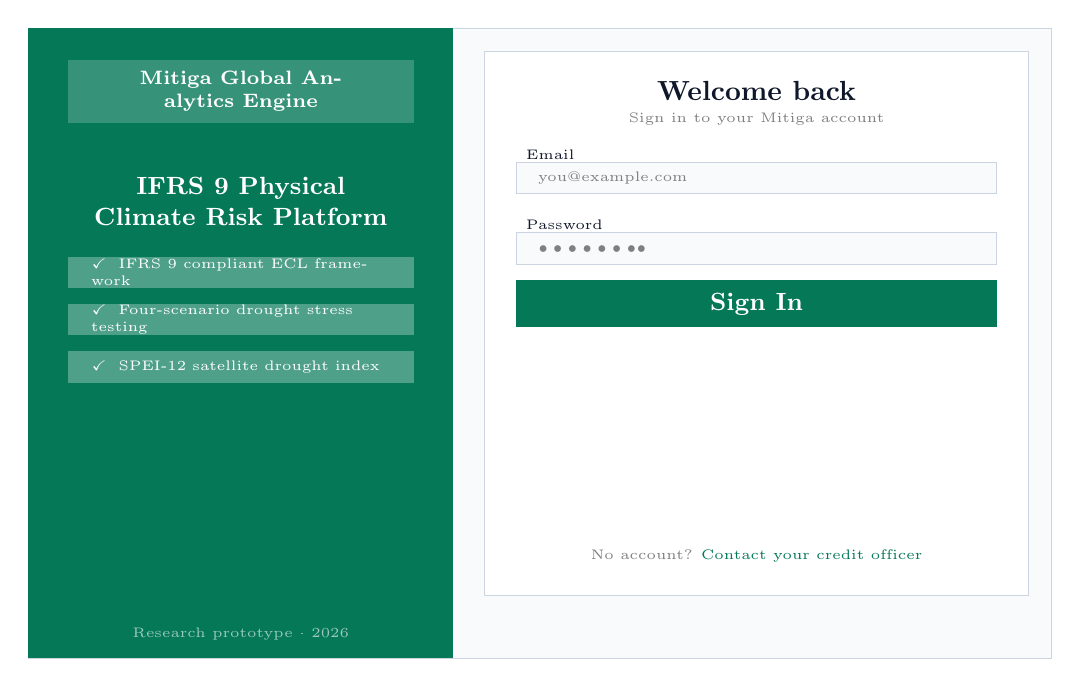
\begin{tikzpicture}[x=1cm, y=1cm]
% ---- outer frame ----
\fill[wfgray] (0,0) rectangle (13,8);
\draw[wfborder] (0,0) rectangle (13,8);

% ---- left green panel ----
\fill[wfgreen] (0,0) rectangle (5.4,8);

% logo area
\fill[white!20!wfgreen] (0.5,6.8) rectangle (4.9,7.6);
\node[white, font=\scriptsize\bfseries, align=center, text width=4cm]
  at (2.7,7.2) {Mitiga Global Analytics Engine};

% heading
\node[white, font=\small\bfseries, align=center, text width=4.2cm]
  at (2.7,5.8) {IFRS 9 Physical\\Climate Risk Platform};

% bullets
\fill[white!30!wfgreen] (0.5,4.7) rectangle (4.9,5.1);
\node[white, font=\tiny, align=left, text width=3.8cm]
  at (2.7,4.9) {$\checkmark$\; IFRS 9 compliant ECL framework};
\fill[white!30!wfgreen] (0.5,4.1) rectangle (4.9,4.5);
\node[white, font=\tiny, align=left, text width=3.8cm]
  at (2.7,4.3) {$\checkmark$\; Four-scenario drought stress testing};
\fill[white!30!wfgreen] (0.5,3.5) rectangle (4.9,3.9);
\node[white, font=\tiny, align=left, text width=3.8cm]
  at (2.7,3.7) {$\checkmark$\; SPEI-12 satellite drought index};

% footer
\node[white!60!wfgreen, font=\tiny] at (2.7,0.3) {Research prototype · 2026};

% ---- right white card ----
\fill[white] (5.8,0.8) rectangle (12.7,7.7);
\draw[wfborder] (5.8,0.8) rectangle (12.7,7.7);

% title
\node[font=\normalsize\bfseries, color=wfdark] at (9.25,7.2) {Welcome back};
\node[font=\tiny, color=gray]                  at (9.25,6.85){Sign in to your Mitiga account};

% email
\node[font=\tiny, anchor=west, color=wfdark]   at (6.2,6.4)  {Email};
\fill[wfgray] (6.2,5.9) rectangle (12.3,6.3);
\draw[wfborder] (6.2,5.9) rectangle (12.3,6.3);
\node[font=\tiny, color=gray, anchor=west]     at (6.35,6.1) {you@example.com};

% password
\node[font=\tiny, anchor=west, color=wfdark]   at (6.2,5.5)  {Password};
\fill[wfgray] (6.2,5.0) rectangle (12.3,5.4);
\draw[wfborder] (6.2,5.0) rectangle (12.3,5.4);
\node[font=\tiny, color=gray, anchor=west]     at (6.35,5.2) {$\bullet\bullet\bullet\bullet\bullet\bullet\bullet\bullet$};

% button
\fill[wfgreen] (6.2,4.2) rectangle (12.3,4.8);
\node[white, font=\small\bfseries]             at (9.25,4.5) {Sign In};

% footer link
\draw[wfborder] (5.8,0.8) -- (12.7,0.8);
\node[font=\tiny, color=gray]                  at (9.25,1.3)
  {No account? \textcolor{wfgreen}{Contact your credit officer}};
\end{tikzpicture}
\caption{Login Page}
\label{fig:login}
\end{figure}

The login page is the entry point for all users. It accepts an email address and password. After successful login, the system reads the user's role from the database. Administrators are redirected to the admin dashboard. Borrowers go to their personal dashboard. The left panel of the page shows the system name and three feature highlights: IFRS 9 compliance, four-scenario drought stress testing, and the SPEI-12 satellite drought index. This gives a visitor a clear picture of what the system does before they even sign in.

% ----------------------------------------------------------
% 3.3.2  LANDING PAGE
% ----------------------------------------------------------
\subsection{Landing Page}

\begin{figure}[H]
\centering
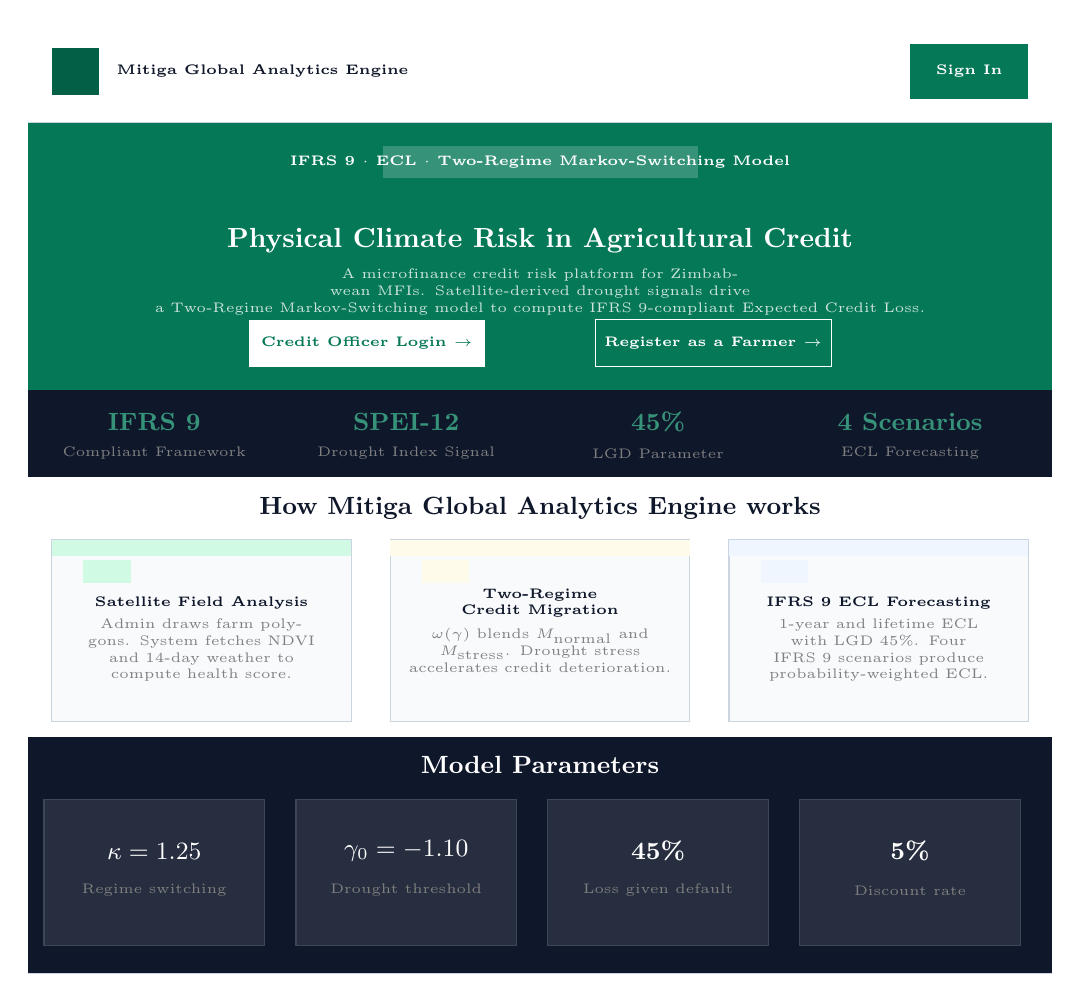
\begin{tikzpicture}[x=1cm, y=1cm]
% outer frame
\fill[wfgray] (0,0) rectangle (13,12);
\draw[wfborder] (0,0) rectangle (13,12);

% ---- navbar ----
\fill[white] (0,10.8) rectangle (13,12);
\draw[wfborder] (0,10.8) -- (13,10.8);
\fill[wfgreen!80!black] (0.3,11.15) rectangle (0.9,11.75);
\node[font=\tiny\bfseries, color=wfdark, anchor=west] at (1.0,11.45)
  {Mitiga Global Analytics Engine};
\fill[wfgreen] (11.2,11.1) rectangle (12.7,11.8);
\node[white, font=\tiny\bfseries] at (11.95,11.45) {Sign In};

% ---- hero section ----
\fill[wfgreen] (0,7.4) rectangle (13,10.8);
% IFRS badge
\fill[white!20!wfgreen] (4.5,10.1) rectangle (8.5,10.5);
\node[white, font=\tiny\bfseries] at (6.5,10.3)
  {IFRS 9 $\cdot$ ECL $\cdot$ Two-Regime Markov-Switching Model};
% title
\node[white, font=\normalsize\bfseries, align=center, text width=10cm]
  at (6.5,9.3) {Physical Climate Risk in Agricultural Credit};
\node[white!80!wfgreen, font=\tiny, align=center, text width=10cm]
  at (6.5,8.65)
  {A microfinance credit risk platform for Zimbabwean MFIs. Satellite-derived drought signals drive\\a Two-Regime Markov-Switching model to compute IFRS 9-compliant Expected Credit Loss.};
% CTA buttons
\fill[white] (2.8,7.7) rectangle (5.8,8.3);
\node[wfgreen, font=\tiny\bfseries] at (4.3,8.0) {Credit Officer Login $\rightarrow$};
\draw[white] (7.2,7.7) rectangle (10.2,8.3);
\node[white, font=\tiny\bfseries] at (8.7,8.0) {Register as a Farmer $\rightarrow$};

% ---- stats strip ----
\fill[wfdark] (0,6.3) rectangle (13,7.4);
\foreach \x/\v/\l in {1.6/IFRS 9/Compliant Framework, 4.8/SPEI-12/Drought Index Signal,
                       8.0/45\%/LGD Parameter, 11.2/4 Scenarios/ECL Forecasting}{
  \node[font=\small\bfseries, color=wfgreen!80] at (\x,7.0) {\v};
  \node[font=\tiny, color=gray]                 at (\x,6.6) {\l};
}

% ---- feature cards ----
\fill[white] (0,3.0) rectangle (13,6.3);
\node[wfdark, font=\small\bfseries] at (6.5,5.9) {How Mitiga Global Analytics Engine works};
% card 1
\fill[wfgray] (0.3,3.2) rectangle (4.1,5.5);
\draw[wfborder] (0.3,3.2) rectangle (4.1,5.5);
\fill[wfgreenlt] (0.3,5.3) rectangle (4.1,5.5);
\fill[wfgreenlt] (0.7,4.95) rectangle (1.3,5.25);
\node[font=\tiny\bfseries, wfdark, align=center, text width=3.5cm] at (2.2,4.7)
  {Satellite Field Analysis};
\node[font=\tiny, color=gray, align=center, text width=3.4cm] at (2.2,4.1)
  {Admin draws farm polygons. System fetches NDVI and 14-day weather to compute health score.};
% card 2
\fill[wfgray] (4.6,3.2) rectangle (8.4,5.5);
\draw[wfborder] (4.6,3.2) rectangle (8.4,5.5);
\fill[wfamber] (4.6,5.3) rectangle (8.4,5.5);
\fill[wfamber] (5.0,4.95) rectangle (5.6,5.25);
\node[font=\tiny\bfseries, wfdark, align=center, text width=3.5cm] at (6.5,4.7)
  {Two-Regime Credit Migration};
\node[font=\tiny, color=gray, align=center, text width=3.4cm] at (6.5,4.1)
  {$\omega(\gamma)$ blends $\Mnormal$ and $\Mstress$. Drought stress accelerates credit deterioration.};
% card 3
\fill[wfgray] (8.9,3.2) rectangle (12.7,5.5);
\draw[wfborder] (8.9,3.2) rectangle (12.7,5.5);
\fill[wfblue] (8.9,5.3) rectangle (12.7,5.5);
\fill[wfblue] (9.3,4.95) rectangle (9.9,5.25);
\node[font=\tiny\bfseries, wfdark, align=center, text width=3.5cm] at (10.8,4.7)
  {IFRS 9 ECL Forecasting};
\node[font=\tiny, color=gray, align=center, text width=3.4cm] at (10.8,4.1)
  {1-year and lifetime ECL with LGD 45\%. Four IFRS 9 scenarios produce probability-weighted ECL.};

% ---- model params strip ----
\fill[wfdark] (0,0) rectangle (13,3.0);
\node[white, font=\small\bfseries] at (6.5,2.65) {Model Parameters};
\foreach \x/\v/\l in {1.6/$\kappa = 1.25$/Regime switching,
                       4.8/$\gamma_0 = -1.10$/Drought threshold,
                       8.0/45\%/Loss given default,
                       11.2/5\%/Discount rate}{
  \fill[white!10!wfdark] (\x-1.4,0.35) rectangle (\x+1.4,2.2);
  \draw[white!20!wfdark]  (\x-1.4,0.35) rectangle (\x+1.4,2.2);
  \node[white, font=\small\bfseries]  at (\x,1.55) {\v};
  \node[gray,  font=\tiny]            at (\x,1.05) {\l};
}
\end{tikzpicture}
\caption{Landing Page}
\label{fig:landing}
\end{figure}

The landing page is publicly accessible. It explains the system at a high level. The hero section at the top has two buttons: one for credit officer login and one for farmer self-registration. Below that, three cards summarise the three main functions of the system. A statistics strip shows four headline metrics. The dark parameter section at the bottom makes it clear that this is not a generic risk tool --- it implements specific, calibrated values from the research.

% ----------------------------------------------------------
% 3.3.3  ADMIN DASHBOARD
% ----------------------------------------------------------
\subsection{Admin Dashboard}

\begin{figure}[H]
\centering
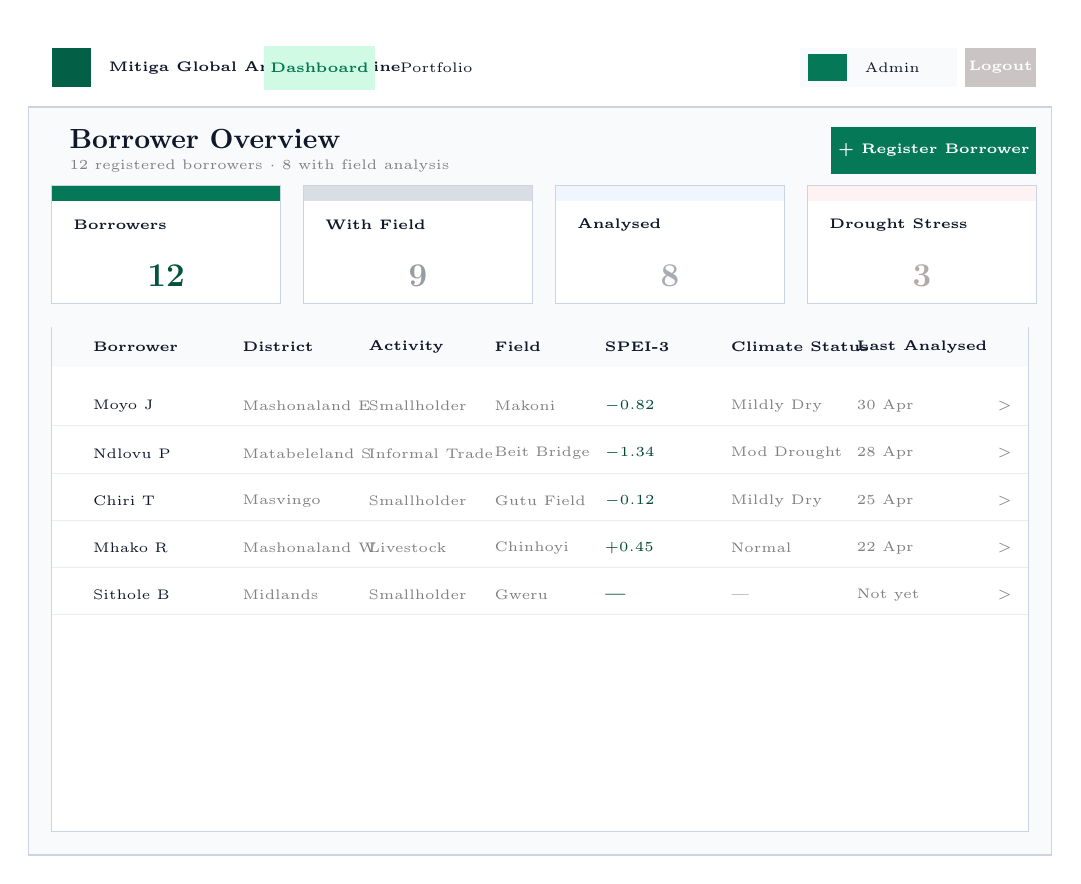
\begin{tikzpicture}[x=1cm, y=1cm]
% outer
\fill[wfgray] (0,0) rectangle (13,10.5);
\draw[wfborder] (0,0) rectangle (13,10.5);

% navbar
\fill[white] (0,9.5) rectangle (13,10.5);
\draw[wfborder] (0,9.5) -- (13,9.5);
\fill[wfgreen!80!black] (0.3,9.75) rectangle (0.8,10.25);
\node[wfdark, font=\tiny\bfseries, anchor=west] at (0.9,10.0)
  {Mitiga Global Analytics Engine};
\fill[wfgreenlt] (3.0,9.72) rectangle (4.4,10.28);
\node[wfgreen,  font=\tiny\bfseries] at (3.7,10.0) {Dashboard};
\node[wfdark,   font=\tiny, anchor=west] at (4.6,10.0) {Portfolio};
% admin badge
\fill[wfgray] (9.8,9.75) rectangle (11.8,10.25);
\fill[wfgreen] (9.9,9.83) rectangle (10.4,10.17);
\node[wfdark, font=\tiny, anchor=west] at (10.5,10.0) {Admin};
\fill[wfred!60!gray] (11.9,9.75) rectangle (12.8,10.25);
\node[white, font=\tiny\bfseries] at (12.35,10.0) {Logout};

% page header
\node[wfdark, font=\normalsize\bfseries, anchor=west] at (0.4,9.1)
  {Borrower Overview};
\node[gray, font=\tiny, anchor=west] at (0.4,8.75)
  {12 registered borrowers $\cdot$ 8 with field analysis};
\fill[wfgreen] (10.2,8.65) rectangle (12.8,9.25);
\node[white, font=\tiny\bfseries] at (11.5,8.95) {+ Register Borrower};

% ---- 4 summary cards ----
\foreach \x/\lbl/\val/\col in {
    0.3/Borrowers/12/wfgreen,
    3.5/{With Field}/9/wfblue!80!gray,
    6.7/Analysed/8/wfblue,
    9.9/{Drought Stress}/3/wfred}{
  \fill[white] (\x,7.0) rectangle (\x+2.9,8.5);
  \draw[wfborder] (\x,7.0) rectangle (\x+2.9,8.5);
  \fill[\col] (\x,8.3) rectangle (\x+2.9,8.5);
  \node[wfdark, font=\tiny\bfseries, anchor=west] at (\x+0.15,8.0) {\lbl};
  \node[\col!70!black, font=\large\bfseries] at (\x+1.45,7.35) {\val};
}

% ---- table ----
\fill[white] (0.3,0.3) rectangle (12.7,6.7);
\draw[wfborder] (0.3,0.3) rectangle (12.7,6.7);
% table header
\fill[wfgray] (0.3,6.2) rectangle (12.7,6.7);
\foreach \x/\h in {0.7/Borrower, 2.6/District, 4.2/Activity,
                    5.8/Field, 7.2/{SPEI-3}, 8.8/{Climate Status},
                    10.4/{Last Analysed}}{
  \node[wfdark, font=\tiny\bfseries, anchor=west] at (\x,6.45) {\h};
}
% table rows — written out manually to avoid \fi conflict
\def\drawrow#1#2#3#4#5#6#7#8{%
  \draw[wfborder!40] (0.3,#1-0.25) -- (12.7,#1-0.25);
  \node[wfdark, font=\tiny, anchor=west] at (0.7,#1) {#2};
  \node[gray,   font=\tiny, anchor=west] at (2.6,#1) {#3};
  \node[gray,   font=\tiny, anchor=west] at (4.2,#1) {#4};
  \node[gray,   font=\tiny, anchor=west] at (5.8,#1) {#5};
  \node[wfgreen!60!black, font=\tiny\bfseries, anchor=west] at (7.2,#1) {#6};
  \node[gray,   font=\tiny, anchor=west] at (8.8,#1) {#7};
  \node[gray,   font=\tiny, anchor=west] at (10.4,#1) {#8};
  \node[gray,   font=\tiny]              at (12.4,#1) {$>$};
}
\drawrow{5.7}{Moyo J}{Mashonaland E}{Smallholder}{Makoni}{$-0.82$}{Mildly Dry}{30 Apr}
\drawrow{5.1}{Ndlovu P}{Matabeleland S}{Informal Trade}{Beit Bridge}{$-1.34$}{Mod Drought}{28 Apr}
\drawrow{4.5}{Chiri T}{Masvingo}{Smallholder}{Gutu Field}{$-0.12$}{Mildly Dry}{25 Apr}
\drawrow{3.9}{Mhako R}{Mashonaland W}{Livestock}{Chinhoyi}{$+0.45$}{Normal}{22 Apr}
\drawrow{3.3}{Sithole B}{Midlands}{Smallholder}{Gweru}{---}{---}{Not yet}
\end{tikzpicture}
\caption{Admin Dashboard}
\label{fig:admin_dashboard}
\end{figure}

The admin dashboard is the main working screen for credit officers. The four summary cards at the top give a quick overview of the portfolio state. The drought stress card is highlighted in red and shows the count of borrowers whose SPEI gamma is below $-1.0$ --- the threshold where the research shows default probabilities increase sharply. The borrower table below shows the full list. Each row has the SPEI-3 gamma value and a climate status label. Clicking the arrow on any row opens the detailed borrower profile.

% ----------------------------------------------------------
% 3.3.4  REGISTER BORROWER
% ----------------------------------------------------------
\subsection{Register Borrower}

\begin{figure}[H]
\centering
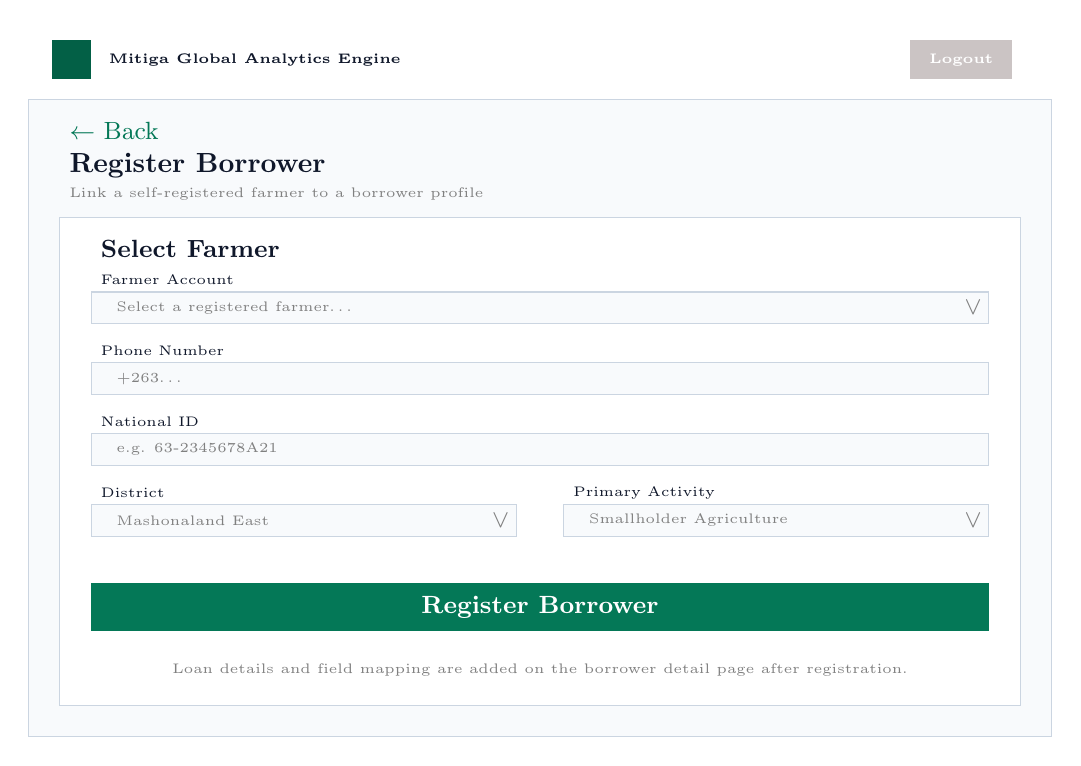
\begin{tikzpicture}[x=1cm, y=1cm]
% outer
\fill[wfgray] (0,0) rectangle (13,9);
\draw[wfborder] (0,0) rectangle (13,9);

% navbar
\fill[white] (0,8.1) rectangle (13,9);
\draw[wfborder] (0,8.1) -- (13,8.1);
\fill[wfgreen!80!black] (0.3,8.35) rectangle (0.8,8.85);
\node[wfdark, font=\tiny\bfseries, anchor=west] at (0.9,8.6) {Mitiga Global Analytics Engine};
\fill[wfred!60!gray] (11.2,8.35) rectangle (12.5,8.85);
\node[white, font=\tiny\bfseries] at (11.85,8.6) {Logout};

% back + title
\node[wfgreen, font=\small, anchor=west] at (0.4,7.7) {$\leftarrow$ Back};
\node[wfdark, font=\normalsize\bfseries, anchor=west] at (0.4,7.25){Register Borrower};
\node[gray,   font=\tiny, anchor=west]    at (0.4,6.9) {Link a self-registered farmer to a borrower profile};

% card
\fill[white] (0.4,0.4) rectangle (12.6,6.6);
\draw[wfborder] (0.4,0.4) rectangle (12.6,6.6);

% section label
\node[wfdark, font=\small\bfseries, anchor=west] at (0.8,6.2) {Select Farmer};

% farmer dropdown
\node[wfdark, font=\tiny, anchor=west] at (0.8,5.8) {Farmer Account};
\fill[wfgray]  (0.8,5.25) rectangle (12.2,5.65);
\draw[wfborder](0.8,5.25) rectangle (12.2,5.65);
\node[gray, font=\tiny, anchor=west]  at (1.0,5.45) {Select a registered farmer\ldots};
\node[gray, font=\small]              at (12.0,5.45) {$\vee$};

% phone
\node[wfdark, font=\tiny, anchor=west] at (0.8,4.9) {Phone Number};
\fill[wfgray]  (0.8,4.35) rectangle (12.2,4.75);
\draw[wfborder](0.8,4.35) rectangle (12.2,4.75);
\node[gray, font=\tiny, anchor=west] at (1.0,4.55) {+263\ldots};

% national ID
\node[wfdark, font=\tiny, anchor=west] at (0.8,4.0) {National ID};
\fill[wfgray]  (0.8,3.45) rectangle (12.2,3.85);
\draw[wfborder](0.8,3.45) rectangle (12.2,3.85);
\node[gray, font=\tiny, anchor=west] at (1.0,3.65) {e.g. 63-2345678A21};

% district + activity side by side
\node[wfdark, font=\tiny, anchor=west] at (0.8,3.1) {District};
\fill[wfgray]  (0.8,2.55) rectangle (6.2,2.95);
\draw[wfborder](0.8,2.55) rectangle (6.2,2.95);
\node[gray, font=\tiny, anchor=west] at (1.0,2.75) {Mashonaland East};
\node[gray, font=\small] at (6.0,2.75) {$\vee$};

\node[wfdark, font=\tiny, anchor=west] at (6.8,3.1) {Primary Activity};
\fill[wfgray]  (6.8,2.55) rectangle (12.2,2.95);
\draw[wfborder](6.8,2.55) rectangle (12.2,2.95);
\node[gray, font=\tiny, anchor=west] at (7.0,2.75) {Smallholder Agriculture};
\node[gray, font=\small] at (12.0,2.75) {$\vee$};

% register button
\fill[wfgreen] (0.8,1.35) rectangle (12.2,1.95);
\node[white, font=\small\bfseries] at (6.5,1.65) {Register Borrower};

% note
\node[gray, font=\tiny] at (6.5,0.85)
  {Loan details and field mapping are added on the borrower detail page after registration.};
\end{tikzpicture}
\caption{Register Borrower}
\label{fig:register_borrower}
\end{figure}

New borrowers are added to the portfolio by the admin. The registration page shows a dropdown of farmers who have signed up through the public registration page. The admin selects the farmer and fills in the remaining profile details: phone number, national ID, district, and primary economic activity. This two-step design means basic account creation is open to farmers, but sensitive borrower profiling and loan data stays under admin control. The district dropdown covers all eight Zimbabwean provinces that fall within the research's geographic scope.

% ----------------------------------------------------------
% 3.3.5  BORROWER DETAIL AND FIELD ANALYSIS
% ----------------------------------------------------------
\subsection{Borrower Detail and Field Analysis}

\begin{figure}[H]
\centering
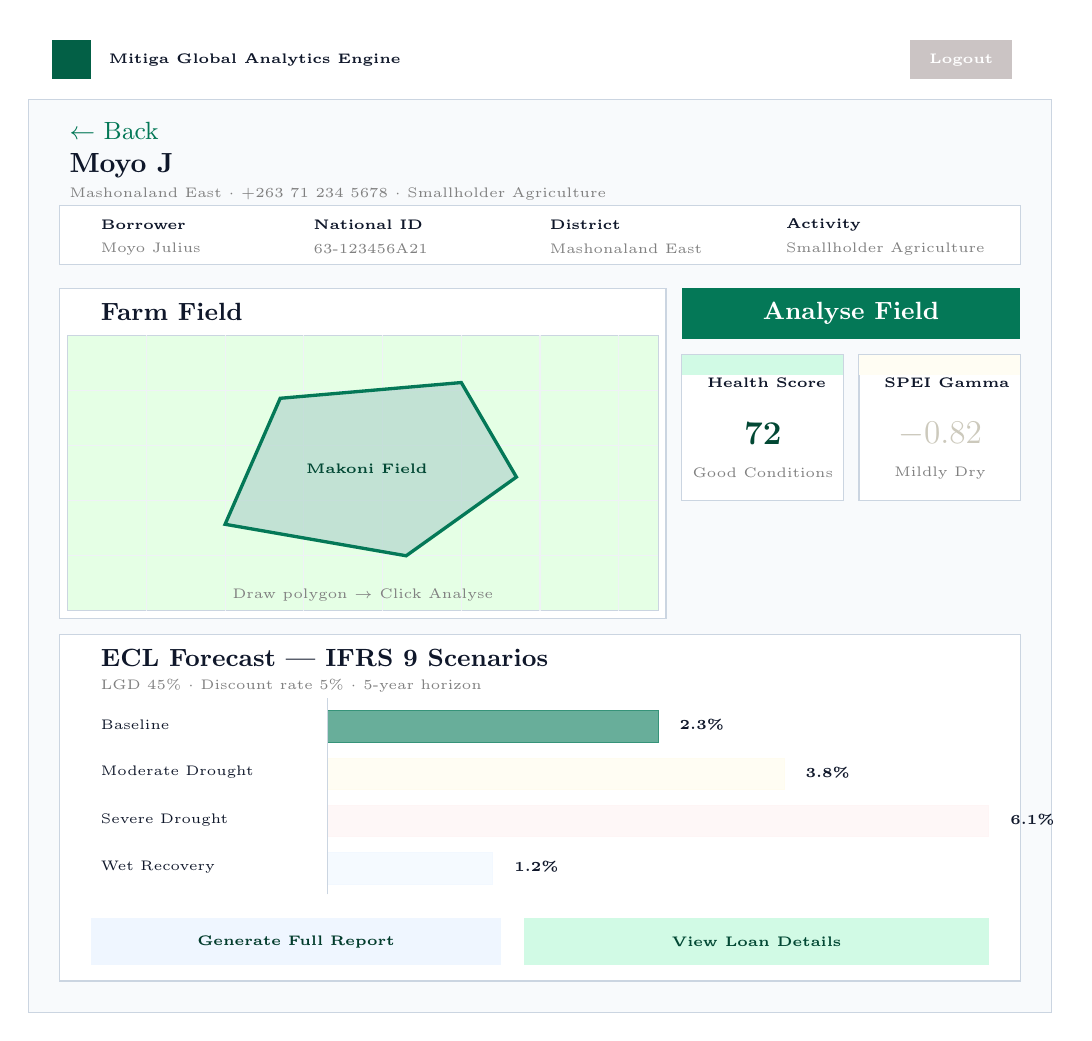
\begin{tikzpicture}[x=1cm, y=1cm]
% outer
\fill[wfgray] (0,0) rectangle (13,12.5);
\draw[wfborder] (0,0) rectangle (13,12.5);

% navbar
\fill[white] (0,11.6) rectangle (13,12.5);
\draw[wfborder] (0,11.6) -- (13,11.6);
\fill[wfgreen!80!black] (0.3,11.85) rectangle (0.8,12.35);
\node[wfdark, font=\tiny\bfseries, anchor=west] at (0.9,12.1) {Mitiga Global Analytics Engine};
\fill[wfred!60!gray] (11.2,11.85) rectangle (12.5,12.35);
\node[white, font=\tiny\bfseries] at (11.85,12.1) {Logout};

% back + name
\node[wfgreen, font=\small, anchor=west] at (0.4,11.2) {$\leftarrow$ Back};
\node[wfdark, font=\normalsize\bfseries, anchor=west] at (0.4,10.75){Moyo J};
\node[gray, font=\tiny, anchor=west] at (0.4,10.4)
  {Mashonaland East $\cdot$ +263 71 234 5678 $\cdot$ Smallholder Agriculture};

% ---- profile info row ----
\fill[white] (0.4,9.5) rectangle (12.6,10.25);
\draw[wfborder] (0.4,9.5) rectangle (12.6,10.25);
\node[wfdark, font=\tiny\bfseries, anchor=west] at (0.8,10.0) {Borrower};
\node[gray, font=\tiny, anchor=west]  at (0.8,9.7)  {Moyo Julius};
\node[wfdark, font=\tiny\bfseries, anchor=west] at (3.5,10.0) {National ID};
\node[gray, font=\tiny, anchor=west]  at (3.5,9.7)  {63-123456A21};
\node[wfdark, font=\tiny\bfseries, anchor=west] at (6.5,10.0) {District};
\node[gray, font=\tiny, anchor=west]  at (6.5,9.7)  {Mashonaland East};
\node[wfdark, font=\tiny\bfseries, anchor=west] at (9.5,10.0) {Activity};
\node[gray, font=\tiny, anchor=west]  at (9.5,9.7)  {Smallholder Agriculture};

% ---- farm map card ----
\fill[white] (0.4,5.0) rectangle (8.1,9.2);
\draw[wfborder] (0.4,5.0) rectangle (8.1,9.2);
\node[wfdark, font=\small\bfseries, anchor=west] at (0.8,8.9) {Farm Field};
% map placeholder with polygon
\fill[green!10] (0.5,5.1) rectangle (8.0,8.6);
\draw[wfborder] (0.5,5.1) rectangle (8.0,8.6);
% tile grid lines
\foreach \xx in {1.5,2.5,3.5,4.5,5.5,6.5,7.5}{\draw[wfborder!30] (\xx,5.1) -- (\xx,8.6);}
\foreach \yy in {5.8,6.5,7.2,7.9}{\draw[wfborder!30] (0.5,\yy) -- (8.0,\yy);}
% farm polygon
\fill[wfgreen!30, opacity=0.7]
  (2.5,6.2) -- (4.8,5.8) -- (6.2,6.8) -- (5.5,8.0) -- (3.2,7.8) -- cycle;
\draw[wfgreen, very thick]
  (2.5,6.2) -- (4.8,5.8) -- (6.2,6.8) -- (5.5,8.0) -- (3.2,7.8) -- cycle;
\node[wfgreen!60!black, font=\tiny\bfseries] at (4.3,6.9) {Makoni Field};
% map attribution
\node[gray, font=\tiny] at (4.25,5.3) {Draw polygon $\rightarrow$ Click Analyse};

% ---- analyse button ----
\fill[wfgreen] (8.3,8.55) rectangle (12.6,9.2);
\node[white, font=\small\bfseries] at (10.45,8.88) {Analyse Field};

% ---- health + gamma cards ----
\fill[white] (8.3,6.5) rectangle (10.35,8.35);
\draw[wfborder] (8.3,6.5) rectangle (10.35,8.35);
\fill[wfgreenlt] (8.3,8.1) rectangle (10.35,8.35);
\node[wfdark, font=\tiny\bfseries, anchor=west] at (8.5,8.0) {Health Score};
\node[wfgreen!60!black, font=\large\bfseries] at (9.33,7.35) {72};
\node[gray, font=\tiny] at (9.33,6.85) {Good Conditions};

\fill[white] (10.55,6.5) rectangle (12.6,8.35);
\draw[wfborder] (10.55,6.5) rectangle (12.6,8.35);
\fill[wfamber!60] (10.55,8.1) rectangle (12.6,8.35);
\node[wfdark, font=\tiny\bfseries, anchor=west] at (10.75,8.0) {SPEI Gamma};
\node[wfamber!80!black, font=\large\bfseries] at (11.58,7.35) {$-0.82$};
\node[gray, font=\tiny] at (11.58,6.85) {Mildly Dry};

% ---- ECL scenarios ----
\fill[white] (0.4,0.4) rectangle (12.6,4.8);
\draw[wfborder] (0.4,0.4) rectangle (12.6,4.8);
\node[wfdark, font=\small\bfseries, anchor=west] at (0.8,4.5) {ECL Forecast --- IFRS 9 Scenarios};
\node[gray, font=\tiny, anchor=west] at (0.8,4.15) {LGD 45\% $\cdot$ Discount rate 5\% $\cdot$ 5-year horizon};

% scenario bars
\foreach \y/\lbl/\bw/\pct/\col in {
    3.65/Baseline/4.2/2.3\%/wfgreen,
    3.05/{Moderate Drought}/5.8/3.8\%/wfamber,
    2.45/{Severe Drought}/8.4/6.1\%/wfred,
    1.85/{Wet Recovery}/2.1/1.2\%/wfblue}{
  \node[wfdark, font=\tiny, anchor=west] at (0.8,\y) {\lbl};
  \fill[\col!60] (3.8,\y-0.22) rectangle (3.8+\bw,\y+0.18);
  \draw[\col!80]  (3.8,\y-0.22) rectangle (3.8+\bw,\y+0.18);
  \node[wfdark, font=\tiny\bfseries, anchor=west] at (3.8+\bw+0.15,\y) {\pct};
}

\draw[wfborder] (3.8,1.5) -- (3.8,4.0);

% report button
\fill[wfblue] (0.8,0.6) rectangle (6.0,1.2);
\node[wfgreen!50!black, font=\tiny\bfseries] at (3.4,0.9) {Generate Full Report};
\fill[wfgreenlt] (6.3,0.6) rectangle (12.2,1.2);
\node[wfgreen!60!black, font=\tiny\bfseries] at (9.25,0.9) {View Loan Details};
\end{tikzpicture}
\caption{Borrower Detail and Field Analysis}
\label{fig:borrower_detail}
\end{figure}

The borrower detail page is where the actual climate risk analysis takes place. The admin draws a polygon on the embedded map to mark the farm boundaries. Clicking Analyse sends the polygon coordinates to the backend, which forwards them to Google Earth Engine. GEE returns NDVI and weather data for that location. The system computes the agricultural health score from five inputs: mean NDVI, NDVI trend, average temperature, total rainfall, and water stress risk. The score maps to a drought gamma value. Gamma determines the regime weight $\omega(\gamma)$, which blends $\Mnormal$ and $\Mstress$ to produce the climate-adjusted PD. ECL is then computed as:
\[
\ECL = \sum_{t=1}^{T} \frac{\PD_t \times \LGD \times \EAD}{(1+r)^t}
\]
with LGD fixed at 45\% and a 5\% annual discount rate, matching the dissertation's calibration.

% ----------------------------------------------------------
% 3.3.6  PORTFOLIO ANALYSIS
% ----------------------------------------------------------
\subsection{Portfolio Analysis}

\begin{figure}[H]
\centering
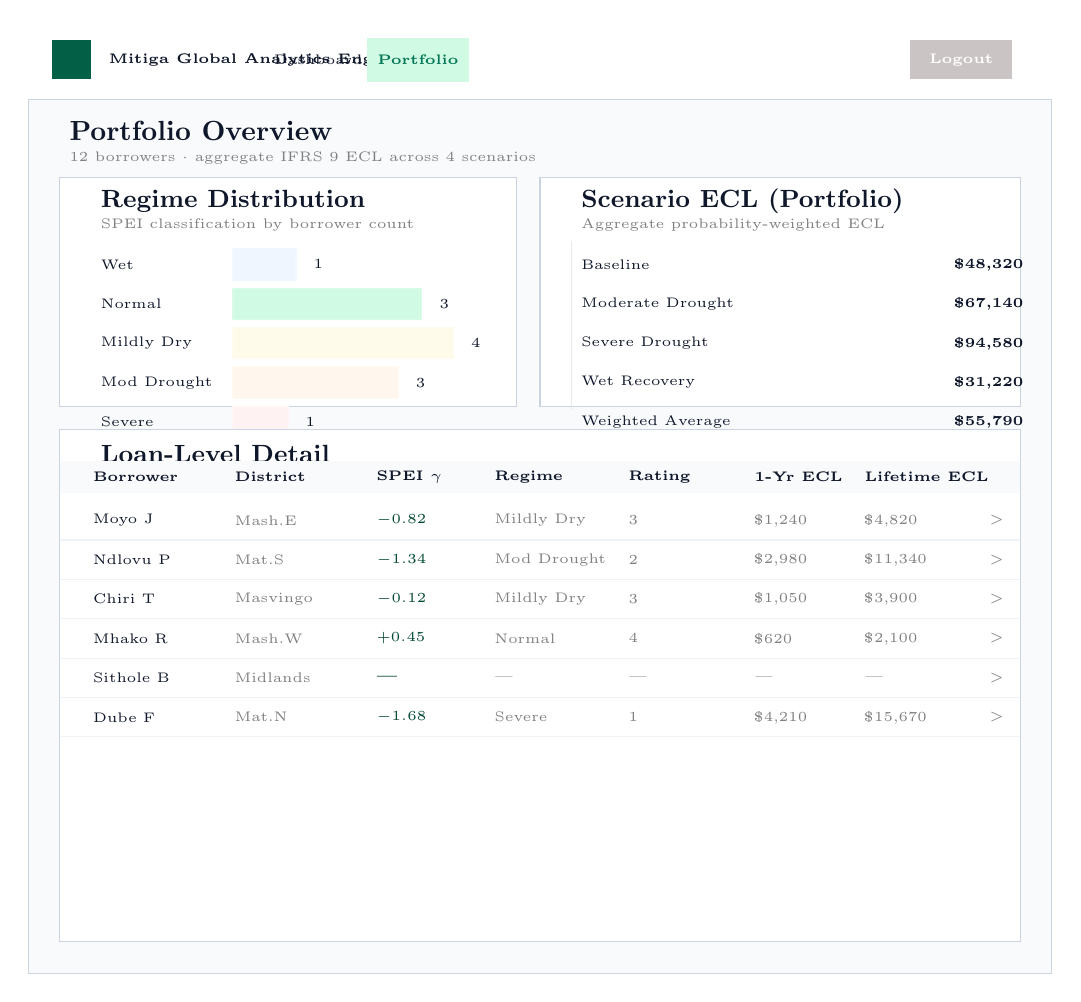
\begin{tikzpicture}[x=1cm, y=1cm]
% outer
\fill[wfgray] (0,0) rectangle (13,12);
\draw[wfborder] (0,0) rectangle (13,12);

% navbar
\fill[white] (0,11.1) rectangle (13,12);
\draw[wfborder] (0,11.1) -- (13,11.1);
\fill[wfgreen!80!black] (0.3,11.35) rectangle (0.8,11.85);
\node[wfdark, font=\tiny\bfseries, anchor=west] at (0.9,11.6) {Mitiga Global Analytics Engine};
\node[wfdark, font=\tiny, anchor=west] at (3.0,11.6) {Dashboard};
\fill[wfgreenlt] (4.3,11.32) rectangle (5.6,11.88);
\node[wfgreen,  font=\tiny\bfseries] at (4.95,11.6) {Portfolio};
\fill[wfred!60!gray] (11.2,11.35) rectangle (12.5,11.85);
\node[white, font=\tiny\bfseries] at (11.85,11.6) {Logout};

% page header
\node[wfdark, font=\normalsize\bfseries, anchor=west] at (0.4,10.7)
  {Portfolio Overview};
\node[gray, font=\tiny, anchor=west] at (0.4,10.35)
  {12 borrowers $\cdot$ aggregate IFRS 9 ECL across 4 scenarios};

% ---- regime distribution ----
\fill[white] (0.4,7.2) rectangle (6.2,10.1);
\draw[wfborder] (0.4,7.2) rectangle (6.2,10.1);
\node[wfdark, font=\small\bfseries, anchor=west] at (0.8,9.8) {Regime Distribution};
\node[gray, font=\tiny, anchor=west] at (0.8,9.5) {SPEI classification by borrower count};

\foreach \y/\lbl/\bw/\cnt/\col in {
    9.0/Wet/0.8/1/wfblue,
    8.5/Normal/2.4/3/wfgreenlt,
    8.0/{Mildly Dry}/2.8/4/wfamber,
    7.5/{Mod Drought}/2.1/3/wfamber!60!wfred,
    7.0/{Severe}/0.7/1/wfred}{
  \node[wfdark, font=\tiny, anchor=west] at (0.8,\y) {\lbl};
  \fill[\col]    (2.6,\y-0.2) rectangle (2.6+\bw,\y+0.2);
  \draw[\col!80] (2.6,\y-0.2) rectangle (2.6+\bw,\y+0.2);
  \node[wfdark, font=\tiny, anchor=west] at (2.6+\bw+0.1,\y) {\cnt};
}

% ---- scenario ECL summary ----
\fill[white] (6.5,7.2) rectangle (12.6,10.1);
\draw[wfborder] (6.5,7.2) rectangle (12.6,10.1);
\node[wfdark, font=\small\bfseries, anchor=west] at (6.9,9.8) {Scenario ECL (Portfolio)};
\node[gray, font=\tiny, anchor=west] at (6.9,9.5) {Aggregate probability-weighted ECL};

\foreach \y/\lbl/\pct/\col in {
    9.0/Baseline/\$48{,}320/wfgreen,
    8.5/{Moderate Drought}/\$67{,}140/wfamber,
    8.0/{Severe Drought}/\$94{,}580/wfred,
    7.5/{Wet Recovery}/\$31{,}220/wfblue,
    7.0/{Weighted Average}/\$55{,}790/wfgreen!60!black}{
  \node[wfdark, font=\tiny, anchor=west] at (6.9,\y) {\lbl};
  \node[wfdark, font=\tiny\bfseries] at (12.2,\y) {\pct};
}
\draw[wfborder!50] (6.9,7.15) -- (6.9,9.3);

% ---- loan table ----
\fill[white] (0.4,0.4) rectangle (12.6,6.9);
\draw[wfborder] (0.4,0.4) rectangle (12.6,6.9);
\node[wfdark, font=\small\bfseries, anchor=west] at (0.8,6.6) {Loan-Level Detail};

% header
\fill[wfgray] (0.4,6.1) rectangle (12.6,6.5);
\foreach \x/\h in {0.7/Borrower, 2.5/District, 4.3/{SPEI $\gamma$},
                    5.8/{Regime}, 7.5/{Rating}, 9.1/{1-Yr ECL},
                    10.5/{Lifetime ECL}}{
  \node[wfdark, font=\tiny\bfseries, anchor=west] at (\x,6.3) {\h};
}

% loan rows — written manually
\def\loanrow#1#2#3#4#5#6#7#8{%
  \draw[wfborder!30] (0.4,#1-0.25) -- (12.6,#1-0.25);
  \node[wfdark, font=\tiny, anchor=west] at (0.7,#1) {#2};
  \node[gray,   font=\tiny, anchor=west] at (2.5,#1) {#3};
  \node[wfgreen!60!black, font=\tiny\bfseries, anchor=west] at (4.3,#1) {#4};
  \node[gray,   font=\tiny, anchor=west] at (5.8,#1) {#5};
  \node[gray,   font=\tiny, anchor=west] at (7.5,#1) {#6};
  \node[gray,   font=\tiny, anchor=west] at (9.1,#1) {#7};
  \node[gray,   font=\tiny, anchor=west] at (10.5,#1) {#8};
  \node[gray,   font=\tiny]              at (12.3,#1) {$>$};
}
\loanrow{5.75}{Moyo J}{Mash.E}{$-0.82$}{Mildly Dry}{3}{\$1,240}{\$4,820}
\loanrow{5.25}{Ndlovu P}{Mat.S}{$-1.34$}{Mod Drought}{2}{\$2,980}{\$11,340}
\loanrow{4.75}{Chiri T}{Masvingo}{$-0.12$}{Mildly Dry}{3}{\$1,050}{\$3,900}
\loanrow{4.25}{Mhako R}{Mash.W}{$+0.45$}{Normal}{4}{\$620}{\$2,100}
\loanrow{3.75}{Sithole B}{Midlands}{---}{---}{---}{---}{---}
\loanrow{3.25}{Dube F}{Mat.N}{$-1.68$}{Severe}{1}{\$4,210}{\$15,670}
\end{tikzpicture}
\caption{Portfolio Analysis}
\label{fig:portfolio}
\end{figure}

The portfolio page aggregates all borrower results into a single view. The regime distribution bars on the left show immediately how much of the portfolio is sitting in drought-stress territory. This is the key early-warning signal for MFI management. If a large fraction of the portfolio is in the moderate or severe drought regime, ECL provisioning needs to go up. The scenario ECL summary on the right shows four aggregate ECL figures for the whole portfolio. The loan table at the bottom gives per-borrower detail so the credit officer can identify the specific accounts driving the highest ECL figures.

% ----------------------------------------------------------
% 3.3.7  BORROWER DASHBOARD
% ----------------------------------------------------------
\subsection{Borrower Dashboard}

\begin{figure}[H]
\centering
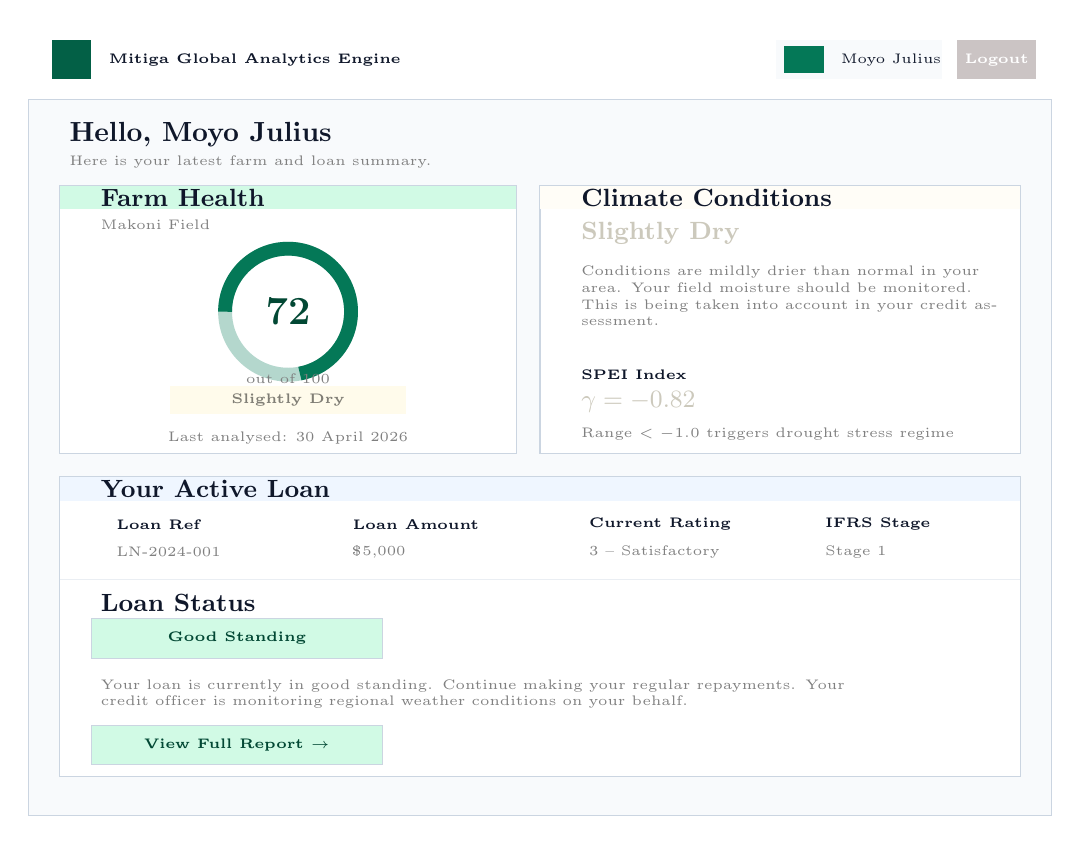
\begin{tikzpicture}[x=1cm, y=1cm]
% outer
\fill[wfgray] (0,0) rectangle (13,10);
\draw[wfborder] (0,0) rectangle (13,10);

% navbar
\fill[white] (0,9.1) rectangle (13,10);
\draw[wfborder] (0,9.1) -- (13,9.1);
\fill[wfgreen!80!black] (0.3,9.35) rectangle (0.8,9.85);
\node[wfdark, font=\tiny\bfseries, anchor=west] at (0.9,9.6) {Mitiga Global Analytics Engine};
\fill[wfgray] (9.5,9.35) rectangle (11.6,9.85);
\fill[wfgreen] (9.6,9.43) rectangle (10.1,9.77);
\node[wfdark, font=\tiny, anchor=west] at (10.2,9.6) {Moyo Julius};
\fill[wfred!60!gray] (11.8,9.35) rectangle (12.8,9.85);
\node[white, font=\tiny\bfseries] at (12.3,9.6) {Logout};

% greeting
\node[wfdark, font=\normalsize\bfseries, anchor=west] at (0.4,8.65)
  {Hello, Moyo Julius};
\node[gray, font=\tiny, anchor=west] at (0.4,8.30)
  {Here is your latest farm and loan summary.};

% ---- farm health card ----
\fill[white] (0.4,4.6) rectangle (6.2,8.0);
\draw[wfborder] (0.4,4.6) rectangle (6.2,8.0);
\fill[wfgreenlt] (0.4,7.7) rectangle (6.2,8.0);
\node[wfdark, font=\small\bfseries, anchor=west] at (0.8,7.85) {Farm Health};
\node[gray, font=\tiny, anchor=west] at (0.8,7.5) {Makoni Field};

% score circle (simulated)
\draw[wfgreen!30, line width=5pt] (3.3,6.4) circle (0.8cm);
\draw[wfgreen,    line width=5pt, rotate around={90:(3.3,6.4)}]
  (3.3,6.4) ++(0,0.8) arc (90:90-0.72*360:0.8cm);
\node[wfgreen!60!black, font=\Large\bfseries] at (3.3,6.4) {72};
\node[gray, font=\tiny] at (3.3,5.55) {out of 100};

% status badge
\fill[wfamber] (1.8,5.1) rectangle (4.8,5.45);
\node[wfamber!50!black, font=\tiny\bfseries] at (3.3,5.28) {Slightly Dry};

\node[gray, font=\tiny] at (3.3,4.8) {Last analysed: 30 April 2026};

% ---- climate card ----
\fill[white] (6.5,4.6) rectangle (12.6,8.0);
\draw[wfborder] (6.5,4.6) rectangle (12.6,8.0);
\fill[wfamber!40] (6.5,7.7) rectangle (12.6,8.0);
\node[wfdark, font=\small\bfseries, anchor=west] at (6.9,7.85) {Climate Conditions};

\node[wfamber!80!black, font=\small\bfseries, anchor=west] at (6.9,7.4)
  {Slightly Dry};
\node[gray, font=\tiny, align=left, text width=5.5cm, anchor=north west]
  at (6.9,7.1)
  {Conditions are mildly drier than normal in your area. Your field moisture should be monitored. This is being taken into account in your credit assessment.};

% SPEI indicator
\node[wfdark, font=\tiny\bfseries, anchor=west] at (6.9,5.6) {SPEI Index};
\node[wfamber!80!black, font=\small\bfseries, anchor=west] at (6.9,5.25) {$\gamma = -0.82$};
\node[gray, font=\tiny, anchor=west] at (6.9,4.85) {Range $< -1.0$ triggers drought stress regime};

% ---- loan card ----
\fill[white] (0.4,0.5) rectangle (12.6,4.3);
\draw[wfborder] (0.4,0.5) rectangle (12.6,4.3);
\fill[wfblue] (0.4,4.0) rectangle (12.6,4.3);
\node[wfdark, font=\small\bfseries, anchor=west] at (0.8,4.15) {Your Active Loan};

\foreach \x/\lbl/\val in {
    1.0/Loan Ref/LN-2024-001,
    4.0/{Loan Amount}/\$5{,}000,
    7.0/{Current Rating}/3 -- Satisfactory,
    10.0/{IFRS Stage}/Stage 1}{
  \node[wfdark, font=\tiny\bfseries, anchor=west] at (\x,3.7) {\lbl};
  \node[gray,   font=\tiny, anchor=west]          at (\x,3.35) {\val};
}

\draw[wfborder!40] (0.4,3.0) -- (12.6,3.0);

\node[wfdark, font=\small\bfseries, anchor=west] at (0.8,2.7) {Loan Status};
\fill[wfgreenlt] (0.8,2.0) rectangle (4.5,2.5);
\draw[wfborder]  (0.8,2.0) rectangle (4.5,2.5);
\node[wfgreen!60!black, font=\tiny\bfseries] at (2.65,2.25) {Good Standing};

\node[gray, font=\tiny, align=left, text width=10cm, anchor=north west]
  at (0.8,1.85)
  {Your loan is currently in good standing. Continue making your regular repayments. Your credit officer is monitoring regional weather conditions on your behalf.};

% report link
\fill[wfgreenlt] (0.8,0.65) rectangle (4.5,1.15);
\draw[wfborder]  (0.8,0.65) rectangle (4.5,1.15);
\node[wfgreen!60!black, font=\tiny\bfseries] at (2.65,0.9) {View Full Report $\rightarrow$};
\end{tikzpicture}
\caption{Borrower Dashboard}
\label{fig:borrower_dashboard}
\end{figure}

The borrower dashboard is designed for farmers, not analysts. It shows none of the model parameters. The farmer sees their farm name, an agricultural health score displayed inside a progress ring, a colour-coded status badge, and a plain-language description of current climate conditions. The loan card below uses simple language to describe the loan status. If conditions worsen, the status badge changes from green to amber to red and the explanatory text updates accordingly. The goal is to keep the farmer informed without overwhelming them with financial terminology.

\subsection*{Conclusion}

The implemented system faithfully translates the research framework into a working application. Each screen has a clear purpose and serves either the credit officer or the farmer. The flowchart in Section 3.2 maps directly to the screens above. From the GEE satellite fetch through to the portfolio ECL summary, every step is traceable back to the Two-Regime Markov-Switching model and the IFRS 9 ECL formula from the dissertation.

\newpage

% ============================================
% APPENDIX
% ============================================
\phantomsection
\addcontentsline{toc}{section}{Appendix: System Code}

\section*{APPENDIX}

\subsection*{System Code}

The following Python scripts form the machine learning pipeline that trains the agricultural health model used inside the Mitiga Global Analytics Engine. The trained model is exported as a JSON file containing the logistic regression coefficients and intercept, which the Next.js server reads at runtime to classify field health without calling an external Python service.

\subsubsection*{config.py}

\begin{lstlisting}[language=Python, caption={config.py --- Project paths and feature configuration}]
import os
from pathlib import Path

# Base Paths
BASE_DIR = Path(__file__).resolve().parent.parent
DATA_DIR = BASE_DIR / "data"
RAW_DATA_PATH = DATA_DIR / "raw" / "dataset.csv"
PROCESSED_DATA_DIR = DATA_DIR / "processed"
MODEL_DIR = BASE_DIR / "models"
REPORT_DIR = BASE_DIR / "reports"

# Ensure directories exist
PROCESSED_DATA_DIR.mkdir(parents=True, exist_ok=True)
MODEL_DIR.mkdir(parents=True, exist_ok=True)
REPORT_DIR.mkdir(parents=True, exist_ok=True)

# Feature Configuration
FEATURES = [
    "mean_ndvi",
    "ndvi_trend",
    "ndvi_variance",
    "avg_temperature_c",
    "total_rainfall_mm"
]
TARGET = "crop_health_label"

# Model Export Path
MODEL_EXPORT_PATH = MODEL_DIR / "crop_health_model.json"
THRESHOLDS_PATH = MODEL_DIR / "thresholds.json"
\end{lstlisting}

\subsubsection*{feature\_engineering.py}

\begin{lstlisting}[language=Python, caption={feature\_engineering.py --- Feature processing logic}]
"""
Feature engineering logic.
In a production app, this would process raw GEE output into
model-ready features such as mean NDVI and rainfall totals.
For this prototype, dataset.csv already contains these features.
"""

def process_features(raw_data):
    # Placeholder for logic that converts raw GEE output to model features
    return raw_data
\end{lstlisting}

\subsubsection*{labeling.py}

\begin{lstlisting}[language=Python, caption={labeling.py --- Rule-based training label generation}]
"""
Labeling logic for training data.
Converts NDVI and weather patterns into 'HEALTHY',
'MODERATE_STRESS', or 'HIGH_STRESS'.
"""

def apply_labels(df):
    # Rule-based labeling used to generate training data
    # if labels were not already present in the dataset.
    return df
\end{lstlisting}

\subsubsection*{train\_health\_model.py}

\begin{lstlisting}[language=Python, caption={train\_health\_model.py --- Logistic Regression training script}]
import pandas as pd
import joblib
from sklearn.model_selection import train_test_split
from sklearn.linear_model import LogisticRegression
from sklearn.metrics import classification_report, confusion_matrix
import matplotlib.pyplot as plt
import seaborn as sns
from config import RAW_DATA_PATH, FEATURES, TARGET, MODEL_DIR, REPORT_DIR

def train_model():
    print(f"Loading data from {RAW_DATA_PATH}...")
    df = pd.read_csv(RAW_DATA_PATH)

    X = df[FEATURES]
    y = df[TARGET]

    X_train, X_test, y_train, y_test = train_test_split(
        X, y, test_size=0.2, random_state=42
    )

    print("Training Logistic Regression Classifier...")
    model = LogisticRegression(max_iter=1000, random_state=42)
    model.fit(X_train, y_train)

    # Evaluation
    y_pred = model.predict(X_test)
    report = classification_report(y_test, y_pred)
    print("\nClassification Report:")
    print(report)

    # Save report
    with open(REPORT_DIR / "training_summary.md", "w") as f:
        f.write("# Training Summary\n\n")
        f.write("## Classification Report\n")
        f.write("```\n")
        f.write(report)
        f.write("```\n")

    # Confusion Matrix Plot
    plt.figure(figsize=(8, 6))
    cm = confusion_matrix(y_test, y_pred)
    sns.heatmap(cm, annot=True, fmt='d', cmap='Blues',
                xticklabels=model.classes_,
                yticklabels=model.classes_)
    plt.title('Confusion Matrix')
    plt.ylabel('Actual')
    plt.xlabel('Predicted')
    plt.savefig(REPORT_DIR / "confusion_matrix.png")

    # Save model (joblib for Python; JSON export handled separately)
    joblib.dump(model, MODEL_DIR / "crop_health_model.joblib")
    print(f"Model saved to {MODEL_DIR / 'crop_health_model.joblib'}")

    return model

if __name__ == "__main__":
    train_model()
\end{lstlisting}

\subsubsection*{export\_model.py}

\begin{lstlisting}[language=Python, caption={export\_model.py --- Exports trained model coefficients to JSON for the Next.js application}]
import json
import joblib
import numpy as np
from config import MODEL_DIR, FEATURES, MODEL_EXPORT_PATH, THRESHOLDS_PATH

def export_model():
    model_path = MODEL_DIR / "crop_health_model.joblib"
    if not model_path.exists():
        print("Model file not found. Please train the model first.")
        return

    print(f"Loading model from {model_path}...")
    model = joblib.load(model_path)

    # Export Logistic Regression coefficients and intercept
    model_data = {
        "model_type": "LogisticRegression",
        "features": FEATURES,
        "classes": model.classes_.tolist(),
        "coefficients": model.coef_.tolist(),
        "intercept": model.intercept_.tolist()
    }

    with open(MODEL_EXPORT_PATH, "w") as f:
        json.dump(model_data, f, indent=2)

    print(f"Model exported to {MODEL_EXPORT_PATH}")

    # Export classification thresholds
    thresholds = {
        "ndvi": {
            "healthy": 0.6,
            "moderate": 0.45
        },
        "rainfall": {
            "low": 20
        },
        "temperature": {
            "high": 30
        }
    }

    with open(THRESHOLDS_PATH, "w") as f:
        json.dump(thresholds, f, indent=2)

    print(f"Thresholds exported to {THRESHOLDS_PATH}")

if __name__ == "__main__":
    export_model()
\end{lstlisting}

\end{document}
